\documentclass[handout]{beamer}
%==============================================================
% Common Beamer Preamble for Course Lectures: Training and Scaling Language Models
%==============================================================

\usepackage[utf8]{inputenc}
\usepackage[T1]{fontenc}
\usepackage{hyperref}
\usepackage{amsmath,amssymb,xcolor,multicol,booktabs,colortbl}
\usepackage{graphicx,listings}
\renewcommand{\figurename}{Figure.}
\renewcommand{\tablename}{Table.}

% ---- TikZ Libraries ----
\usepackage{tikz}
\usetikzlibrary{positioning,arrows.meta,shapes.geometric,calc,fit,backgrounds,decorations.pathreplacing}

% ---- Presentation defaults ----
\setbeamertemplate{navigation symbols}{}
\setbeamersize{text margin left=0.55cm,text margin right=0.55cm}
\setbeamerfont{title}{size=\LARGE,series=\bfseries}
\setbeamerfont{subtitle}{size=\large}

% ---- FontAwesome fallback ----
\IfFileExists{fontawesome5.sty}{%
  \usepackage{fontawesome5}%
}{%
  \providecommand{\faMicrochip}{}%
  \providecommand{\faComments}{}%
  \providecommand{\faTools}{}%
  \providecommand{\faCheckCircle}{}%
  \providecommand{\faExclamationTriangle}{}%
  \providecommand{\faImage}{}%
  \providecommand{\faRobot}{}%
  \providecommand{\faTerminal}{}%
  \providecommand{\faBook}{}%
  \providecommand{\faRedo}{}%
  \providecommand{\faLayerGroup}{}%
  \providecommand{\faCogs}{}%
  \providecommand{\faDatabase}{}%
  \providecommand{\faHdd}{}%
  \providecommand{\faNetworkWired}{}%
}

% ---- Theme Style and Semantic Colors ----
%==============================================================
% Centralized Semantic Color Definitions for LLMs Presentation
%==============================================================

% ---- Base Template / Theme Colors (Aligned with Palette B) ----
\definecolor{themenavy}{RGB}{22,70,102}       % Palette B primary cerulean: #164666
\definecolor{themeblue}{RGB}{22,70,102}       % Primary alias
\definecolor{primarylight}{RGB}{34,92,132}    % Primary light: #225c84
\definecolor{themeteal}{RGB}{0,159,176}       % Accent cyan-teal: #009fb0
\colorlet{main_color}{themenavy}
\colorlet{accent}{themeteal}

\definecolor{accentdark}{RGB}{0,108,120}      % Deep cyan-teal for contrast text
\definecolor{accentlight}{RGB}{56,178,214}    % Slate accent cyan: #38b2d6
\definecolor{leafred}{RGB}{197,93,61}         % Terracotta red for branches/leaves

% ---- Website Panel & Border Neutrals ----
\definecolor{panelbg}{RGB}{237,245,249}       % Course-panel: #edf5f9
\definecolor{panelborder}{RGB}{204,226,238}   % Course-border: #cce2ee

% ---- Code listing style (syntax highlights) ----
\definecolor{deepblue}{RGB}{22,70,102}
\definecolor{deepred}{rgb}{0.6,0,0}
\definecolor{deepgreen}{RGB}{0,135,150}
\definecolor{halfgray}{gray}{0.55}

% ---- Semantic Theme Navy / Cerulean Shades ----
\colorlet{themebluebg}{panelbg}               % Panel #edf5f9
\colorlet{themebluecard}{main_color!8}        % Mild card background fills
\colorlet{themeblueborder}{panelborder}       % Border #cce2ee
\colorlet{themebluemid}{themeteal!60}         % Accent mid-contrast
\colorlet{themebluedraw}{main_color!80}       % Strong outline draws/strokes

% ---- Semantic Secondary Accent Teal Shades ----
\colorlet{accentdarkbg}{themeteal!10}        % Light secondary background fills
\colorlet{accentdarkdraw}{themeteal}         % Secondary outlines/strokes/text/axes

% ---- Functional Colors: Success Green ----
\definecolor{successgreen}{RGB}{55,145,55}
\colorlet{successbg}{successgreen!8}
\colorlet{successdraw}{successgreen!75}

% ---- Functional Colors: Alert Red ----
\definecolor{alertred}{RGB}{197,55,55}
\colorlet{alertbg}{alertred!8}
\colorlet{alertdraw}{alertred!75}

% ---- Functional Colors: Warning Orange ----
\definecolor{warningorange}{RGB}{220,110,30}
\colorlet{warningbg}{warningorange!10}
\colorlet{warningdraw}{warningorange!80}

% ---- Terracotta Red Shades ----
\colorlet{leafredbg}{leafred!12}
\colorlet{leafreddraw}{leafred!80}

% ---- Accent Violet (SWE-bench / observe phases) ----
\definecolor{accentviolet}{RGB}{120,70,180}
\colorlet{accentvioletbg}{accentviolet!10}
\colorlet{accentvioletdraw}{accentviolet!80}

% ---- Post-Training Axis Blue ----
\definecolor{posttrainingblue}{RGB}{40,90,165}
\colorlet{posttrainingbg}{posttrainingblue!8}
\colorlet{posttrainingdraw}{posttrainingblue!75}

% ---- Harness Component Action Green ----
\definecolor{actiongreen}{RGB}{55,145,55}
\colorlet{actiongreenbg}{actiongreen!10}
\colorlet{actiongreendraw}{actiongreen!65}

% ---- Harness Component Persist Olive ----
\definecolor{persistolive}{RGB}{120,135,40}
\colorlet{persistolivebg}{persistolive!12}
\colorlet{persistolivedraw}{persistolive!70}

% ---- Harness Component Observe Violet ----
\colorlet{observevioletbg}{accentvioletbg}
\colorlet{observevioletdraw}{accentvioletdraw}

% ---- Neutrals (Grays/Blacks) ----
\colorlet{neutralbg}{black!4}             % Very light background fills
\colorlet{neutrallight}{black!30}         % Border frames/ticks/dividers
\colorlet{neutraldark}{black!75}          % Main body text/code listing text

% ---- Beamer Block Color Overrides (Premium Terracotta Theme) ----
\setbeamercolor{block title alert}{bg=leafreddraw,fg=white}
\setbeamercolor{block body alert}{bg=leafredbg}
\setbeamercolor{alerted text}{fg=leafreddraw}

\usepackage{../common/style}
\graphicspath{{../common/figs/}{figs/}}

% ---- Code Listing Config ----
\lstset{
  basicstyle=\ttfamily\footnotesize,
  keywordstyle=\bfseries\color{deepblue},
  emphstyle=\ttfamily\color{deepred},
  stringstyle=\color{deepgreen},
  commentstyle=\color{halfgray}\itshape,
  numbers=left, numberstyle=\tiny\color{halfgray},
  backgroundcolor=\color{codebg},
  frame=l, framerule=1.5pt, rulecolor=\color{themeteal},
  xleftmargin=10pt, framexleftmargin=4pt, numbersep=6pt,
  showstringspaces=false, breaklines=true,
  aboveskip=4pt, belowskip=4pt
}

% ---- Image Placeholder Utility ----
\newcommand{\slideimage}[2][3.8cm]{%
  \begin{center}
    \begin{tikzpicture}
      \node[draw=main_color, dashed, very thick, rounded corners,
        fill=themebluebg, minimum width=0.88\linewidth, minimum height=#1,
      text width=0.80\linewidth, align=center, font=\itshape, text=accentdark]
      {\textbf{[ FIGURE / DIAGRAM ]}\\[6pt] #2};
    \end{tikzpicture}
  \end{center}
}

% ---- Concept Highlight Card Utility ----
\newcommand{\conceptcard}[3]{%
  \begin{coursebox}{#1}{#2}#3\end{coursebox}%
}

% ---- Reusable teaching-slide components ----
\newcommand{\learninggoals}[4]{%
  \begin{frame}{What should be clear by the end?}
    \begin{enumerate}
        \setlength{\itemsep}{7pt}
      \item #1
      \item #2
      \item #3
      \item #4
    \end{enumerate}
  \end{frame}
}

\newcommand{\checkpoint}[2]{%
  \begin{frame}{Checkpoint: #1}
    \begin{block}{Think, then compare}
      #2
    \end{block}
  \end{frame}
}

\newcommand{\takeaways}[4]{%
  \begin{frame}{The durable ideas}
    \begin{enumerate}
        \setlength{\itemsep}{8pt}
      \item #1
      \item #2
      \item #3
      \item #4
    \end{enumerate}
  \end{frame}
}

\newcommand{\smallsource}[1]{%
  \vfill\hfill{\tiny\color{neutraldark}Source: #1}
}

% ---- Logo on content frames ----
\newif\ifplacelogo
\placelogotrue
\logo{\ifplacelogo
  \raisebox{-0.3ex}{
\includegraphics[height=0.4cm]{IMT_Atlantique_logo.png}}%
\fi}

\makeatletter
\define@key{beamerframe}{nologo}[true]{%
  \placelogofalse
}
\makeatother

% Fix Beamer bold font warning: substitute undefined T1/cmss/b/n with T1/cmss/bx/n
\DeclareFontShape{T1}{cmss}{b}{n}{<->ssub * cmss/bx/n}{}

% Default Author & Institute metadata
\author[Jonathan Lys]{Jonathan Lys}
\institute[IMT Atlantique]{IMT Atlantique}

% ---- Front Page / Title Slide Macro ----
% Displays Title + IMT Atlantique logo and Brain logo
\newcommand{\makelecturetitle}[1][Training and Scaling Language Models: From First Principles to Efficient Serving]{%
  \placelogofalse
  {
    \setbeamertemplate{footline}{}
    \settitletagline{#1}
    \settitlelogos{%
      \raisebox{-0.5\height}{
\includegraphics[height=1.15cm]{IMT_Atlantique_logo.png}}%
      \hspace{1.2em}%
      \raisebox{-0.5\height}{\includegraphics[height=1.15cm]{brain.pdf}}}
    \begin{frame}[plain]
      \titlepage
    \end{frame}
  }
  \placelogotrue
}

% Section TOC Frame
\AtBeginSection[]{\coursesectiondivider}

\title[TLM -- Session 11]{Session 11: KV-Cached Decoding\\[4pt]
\normalsize\itshape Reuse, Memory Growth, and Exact Autoregressive State}
\date{\today}

\begin{document}
\makelecturetitle
\begin{frame}{Lecture map}
  \tableofcontents
  \vfill
  \begin{block}{Guiding question}
    What can autoregressive decoding reuse exactly, and how does that reuse turn compute into a memory-management problem?
  \end{block}
\end{frame}
\learninggoals
  {Explain the redundant work removed by a KV cache.}
  {Compute cache shapes and memory for MHA, GQA, and MQA.}
  {Reason about decode bandwidth and cache layout.}
  {Test cached generation against a full-prefix reference.}

\section{From full-prefix recomputation to reuse}

\begin{frame}{Naive decoding recomputes the unchanged prefix}
  To generate token $t+1$, a naive decoder runs the model on $x_{0:t}$. The next step runs it again on $x_{0:t+1}$.
  \begin{alertblock}{Repeated work}
    At every layer, keys and values for positions $0\ldots t$ are deterministic functions of unchanged hidden states. Recomputing them cannot change the result.
  \end{alertblock}
  \begin{block}{Cache principle}
    Store past key and value projections once. At the next step, compute projections only for the new token and attend to cached history.
  \end{block}
  \smallsource{Saad Ahmed, KV Cache Explained Intuitively}
\end{frame}

\begin{frame}{Prefill and decode have different shapes}
  \begin{columns}[t]
    \begin{column}{0.47\linewidth}
      \begin{block}{Prefill}
        processes the prompt in parallel\\many query tokens\\large matrix multiplications\\usually compute-efficient
      \end{block}
    \end{column}
    \begin{column}{0.47\linewidth}
      \begin{block}{Decode}
        processes one new token per request\\reads growing KV history\\small matrix operations\\often bandwidth-bound
      \end{block}
    \end{column}
  \end{columns}
  \begin{alertblock}{Do not average them together}
    Time to first token and inter-token latency arise from different workloads and need separate measurements.
  \end{alertblock}
\end{frame}

\begin{frame}{Cached attention at one layer}
  \centering
  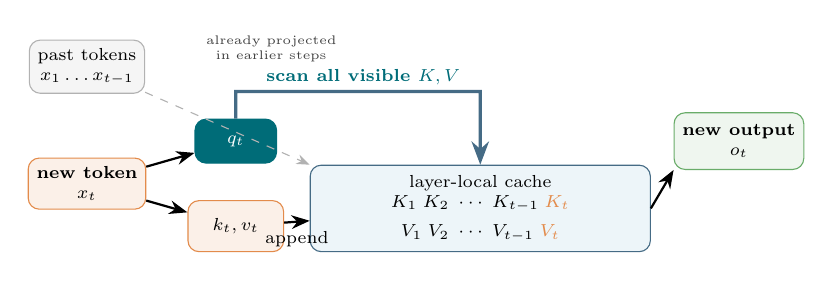
\begin{tikzpicture}[x=1cm,y=1cm,scale=.9,transform shape,every node/.style={font=\scriptsize},
    box/.style={draw=neutrallight,fill=neutralbg,rounded corners,minimum width=1.55cm,minimum height=.72cm,align=center},
    new/.style={draw=warningdraw,fill=warningbg,rounded corners,minimum width=1.35cm,minimum height=.72cm,align=center,font=\scriptsize\bfseries},
    cache/.style={draw=themebluedraw,fill=themebluebg,rounded corners,minimum width=4.8cm,minimum height=1.22cm,align=center}]
    \node[box] (past) at (1.45,3.2) {past tokens\\$x_1\ldots x_{t-1}$};
    \node[new] (xt) at (1.45,1.55) {new token\\$x_t$};
    \node[draw=accentdark,fill=accentdark,text=white,rounded corners,minimum width=1.15cm,minimum height=.62cm,font=\scriptsize\bfseries] (qt) at (3.55,2.15) {$q_t$};
    \node[new] (kvt) at (3.55,.95) {$k_t,v_t$};
    \node[cache] (cache) at (7.0,1.2) {layer-local cache\\\vspace{2pt}$K_1\;K_2\;\cdots\;K_{t-1}\;\color{warningdraw}K_t$\\$V_1\;V_2\;\cdots\;V_{t-1}\;\color{warningdraw}V_t$};
    \node[draw=successdraw,fill=successbg,rounded corners,minimum width=1.65cm,minimum height=.8cm,align=center,font=\scriptsize\bfseries] (out) at (10.65,2.15) {new output\\$o_t$};
    \draw[-{Stealth},thick] (xt)--(qt);
    \draw[-{Stealth},thick] (xt)--(kvt);
    \draw[-{Stealth},thick] (kvt)-- node[below]{append} (cache);
    \draw[-{Stealth},very thick,themebluedraw] (qt.north)--(3.55,2.85)--(7.0,2.85)--(cache.north);
    \node[text=accentdark,font=\scriptsize\bfseries] at (5.35,3.05) {scan all visible $K,V$};
    \draw[-{Stealth},thick] (cache.east)--(out.south west);
    \draw[dashed,neutrallight,-{Stealth}] (past)--(cache.north west);
    \node[font=\tiny,text=neutraldark,align=center] at (4.05,3.45) {already projected\\in earlier steps};
  \end{tikzpicture}
  \vspace{2pt}
  \[
    o_t=\operatorname{softmax}\!\left(q_tK_{1:t}^{\top}/\sqrt{d_h}\right)V_{1:t}
  \]
  \footnotesize The cache removes repeated $K,V$ projection; attention still scans the growing context.
\end{frame}

\begin{frame}{The cache changes asymptotic projection work}
  For $n$ generated tokens after a prompt:
  \begin{columns}[t]
    \begin{column}{0.47\linewidth}
      \begin{alertblock}{Without cache}
        Reproject the growing prefix at every step. Prefix projection work accumulates roughly quadratically in generated length.
      \end{alertblock}
    \end{column}
    \begin{column}{0.47\linewidth}
      \begin{block}{With cache}
        Project each token's key and value once. Attention still scans a context that grows linearly per decode step.
      \end{block}
    \end{column}
  \end{columns}
  \vfill
  \centering The cache removes redundant projection work. It does not make full-context attention constant-time.
\end{frame}

\section{Cache memory and bandwidth}

\begin{frame}{Cache shape determines capacity}
  For $L$ layers, batch $B$, $H_{kv}$ key-value heads, cached length $T$, head width $d_h$, and element size $s$:
  \[
    M_{KV}=2\,L\,B\,H_{kv}\,T\,d_h\,s
  \]
  The factor 2 stores both keys and values.
  \begin{block}{Per-token, per-request growth}
    \[
      m_{\text{token}}=2L H_{kv}d_hs
    \]
    This number links model architecture directly to serving concurrency.
  \end{block}
\end{frame}

\begin{frame}{Worked memory estimate}
  Suppose $L=32$, $H_{kv}=32$, $d_h=128$, BF16, and $T=4096$:
  \[
    M_{KV}=2\cdot32\cdot1\cdot32\cdot4096\cdot128\cdot2
    \approx 2\ \text{GiB}
  \]
  \begin{alertblock}{Serving implication}
    Sixteen concurrent requests at this cached length would need roughly 32 GiB for KV state alone, before weights, workspaces, and fragmentation.
  \end{alertblock}
\end{frame}

\begin{frame}{MHA, GQA, and MQA differ mainly in $H_{kv}$}
  \centering\small
  \begin{tabular}{llll}
    \toprule
    Variant & query heads & KV heads & cache effect \\
    \midrule
    MHA & $H$ & $H$ & baseline \\
    GQA & $H$ & $G$, where $1<G<H$ & reduced by $H/G$ \\
    MQA & $H$ & 1 & reduced by $H$ \\
    \bottomrule
  \end{tabular}
  \vfill
  Query heads share key-value groups while retaining distinct queries. This reduces cache capacity and decode bandwidth at a possible modeling-quality trade-off.
\end{frame}

\begin{frame}{Decode often reads far more bytes than it computes}
  Each new token reads the cached $K,V$ for every active layer and request. Batch-1 decode has little reuse across queries.
  \begin{block}{Bandwidth model}
    \[
      t_{\text{decode}}\gtrsim
      \frac{\text{weight bytes read}+\text{KV bytes read}}{BW_{\text{effective}}}
    \]
  \end{block}
  \begin{alertblock}{Consequence}
    Reducing KV heads, using lower cache precision, batching requests, and improving memory layout can matter more than reducing arithmetic.
  \end{alertblock}
\end{frame}

\begin{frame}{Allocation strategy decides fragmentation and copy cost}
  \begin{columns}[t]
    \begin{column}{0.31\linewidth}
      \begin{block}{Concatenate}
        simple\\repeated allocation and copying\\poor for long generation
      \end{block}
    \end{column}
    \begin{column}{0.31\linewidth}
      \begin{block}{Preallocate}
        fast append\\reserves maximum length\\internal waste
      \end{block}
    \end{column}
    \begin{column}{0.31\linewidth}
      \begin{block}{Paged}
        non-contiguous blocks\\flexible growth\\mapping metadata
      \end{block}
    \end{column}
  \end{columns}
  \vfill
  Paged layouts make variable-length request lifetimes manageable without requiring one contiguous maximum-size allocation per request.
\end{frame}

\checkpoint{capacity calculation}
  {Recompute the worked example with eight KV heads. How many 4096-token requests fit in 32 GiB if 24 GiB is available for cache after weights and workspaces?}

\section{Correctness and benchmarking}

\begin{frame}{The cache must preserve logical positions}
  \begin{itemize}
    \setlength{\itemsep}{8pt}
    \item The new token uses its absolute or rotary position $t$.
    \item The causal mask covers the valid cached prefix and current token.
    \item Padding and per-request lengths cannot expose uninitialized cache entries.
    \item Reordered or paged blocks must reconstruct the same logical sequence.
  \end{itemize}
  \begin{alertblock}{Common failure}
    Correct key-value values at the wrong positions produce plausible but divergent text.
  \end{alertblock}
\end{frame}

\begin{frame}{Full-prefix decoding is the reference oracle}
  For fixed weights, prompt, and token sequence:
  \begin{enumerate}
    \setlength{\itemsep}{7pt}
    \item run a full-prefix forward pass for each step
    \item run cached prefill plus single-token decode
    \item compare next-token logits at every step
    \item repeat across batch sizes, prompt lengths, and cache boundaries
  \end{enumerate}
  \begin{block}{Then test generation}
    Greedy outputs should match exactly within numerical tolerance. Sampling tests require identical random state and probability inputs.
  \end{block}
\end{frame}

\begin{frame}{Benchmark prefill and decode separately}
  \small
  \begin{tabular}{@{}>{\raggedright\arraybackslash}p{.14\linewidth}>{\raggedright\arraybackslash}p{.44\linewidth}>{\raggedright\arraybackslash}p{.32\linewidth}@{}}
    \toprule
    Phase & Primary metrics & Sweep \\
    \midrule
    prefill & latency, prompt tokens/s, peak memory & prompt length, batch \\
    decode & ms/token, output tokens/s, cache bytes & cached length, batch \\
    end-to-end & TTFT, total latency & prompt/output distribution \\
    \bottomrule
  \end{tabular}
  \vfill
  \begin{alertblock}{Warm and synchronize}
    Kernel compilation, allocation, and asynchronous timing can otherwise dominate or under-report short decode steps.
  \end{alertblock}
\end{frame}

\checkpoint{cache debugging}
  {Cached logits match for short prompts but diverge immediately after a page boundary. Which state and indexing checks isolate layout bugs from positional-encoding bugs?}

\takeaways
  {KV caching reuses past key and value projections exactly.}
  {Cache memory grows with layers, KV heads, requests, cached tokens, head width, and precision.}
  {Decode is commonly bandwidth-bound, so cache architecture and layout shape performance.}
  {Full-prefix logit equivalence is the primary correctness test before benchmarking.}
\end{document}
